\documentclass[ 
    aps,
    prl,
    twocolumn,
    letterpaper, 
    10pt,
    %draft,
    superscriptaddress, 
    showpacs,
    showkeys, 
    notitlepage,
    amsmath, 
    amssymb, 
    floatfix 
]{revtex4-1} 
 
\usepackage{graphicx}% Include figure files
\usepackage{dcolumn}% Align table columns on decimal point
\usepackage{bm}% bold math
\usepackage{color}
\usepackage{amssymb}
\usepackage{amsmath}
\usepackage{hyperref}% add hypertext capabilities

 
\newcommand{\bel}{\begin{equation}}
\newcommand{\eel}{\end{equation}}
\newcommand{\be}{\begin{equation*}}
\newcommand{\ee}{\end{equation*}}
\newcommand{\bal}{\begin{eqnarray}}
\newcommand{\eal}{\end{eqnarray}}
\newcommand{\ba}{\begin{eqnarray*}}
\newcommand{\ea}{\end{eqnarray*}}

\newcommand{\no}{\noindent}

\newcommand{\refeq}[1]{Eq.~(\ref{#1})}
\newcommand{\reffig}[1]{Fig.~\ref{#1}}

\newcommand{\ev}[1]{\langle #1 \rangle}
\newcommand{\ket}[1]{| #1 \rangle}
\newcommand{\bra}[1]{\langle #1 |}
\newcommand{\Ev}[1]{\left\langle #1 \right\rangle}
\newcommand{\Ket}[1]{\left| #1 \right\rangle}
\newcommand{\Bra}[1]{\left\langle #1 \right|}
\newcommand{\+}{^\dagger}
\newcommand{\s}{^\ast}
\newcommand{\Tr}{\text{Tr}\,}

\newcommand{\br}{\mathbf{r}}
\newcommand{\bk}{\mathbf{k}}

\newcommand{\DD}{\mathcal{D}}
\newcommand{\PP}{\mathcal{P}}
\newcommand{\OO}{\mathcal{O}}
\newcommand{\eps}{\varepsilon}

\renewcommand{\d}[1]{\!d#1\,}

\newcommand{\pk}[1]{{\bf \color{blue} #1}}

 


\begin{document} 

%%%%%%%%%%%%%%%%%%%%%%%%%%%%%%%%%%%%%%%%
%%%%%%%%%%%%%%%%%%%%%%%%%%%%%%%%%%%%%%%%
\title{ Quantum network of atom clocks: a possible
implementation with neutral atoms }

\author{P. K\'{o}m\'{a}r}
\affiliation{Physics Department, Harvard University, Cambridge,
MA 02138, USA}

\author{T. Topcu}
\affiliation{Physics Department, Harvard University, Cambridge,
MA 02138, USA}
\affiliation{Department of Physics, University of Nevada, Reno, NV 89557, USA}
\affiliation{ITAMP, Harvard-Smithsonian Center for Astrophysics, Cambridge, MA 02138, USA}

\author{E. M. Kessler}
\affiliation{Physics Department, Harvard University, Cambridge,
MA 02138, USA}
\affiliation{ITAMP, Harvard-Smithsonian Center for Astrophysics, Cambridge, MA 02138, USA}

\author{A. Derevianko}
\affiliation{Physics Department, Harvard University, Cambridge,
MA 02138, USA}
\affiliation{Department of Physics, University of Nevada, Reno, NV 89557, USA}
\affiliation{ITAMP, Harvard-Smithsonian Center for Astrophysics, Cambridge, MA 02138, USA}

\author{V. Vuleti\'{c}}
\affiliation{Department of Physics and Research Laboratory of Electronics,
Massachusetts Institute of Technology, Cambridge, MA 02139, USA}

\author{J. Ye}
\affiliation{JILA, NIST, Department of Physics,  University of Colorado,
Boulder, CO 80309, USA}

\author{M. D. Lukin}
\affiliation{Physics Department, Harvard University, Cambridge,
MA 02138, USA}

% \author{Authors}

\date{\today}


%%%%%%%%%%%%%%%%%%%%%%%%%%%%%%%%%%%%%%%%%%%%%%%%%%%%%%%%%%%%%%%%%%%%%%%%%%%%%%%%%%5
%%%%%%%%%%%%%%%%%%%%%%%%%%%%%%%%%%%%%%%%%%%%%%%%%%%%%%%%%%%%%%%%%%%%%%%%%%%%%%%%%%5
% Abstract
%%%%%%%%%%%%%%%%%%%%%%%%%%%%%%%%%%%%%%%%%%%%%%%%%%%%%%%%%%%%%%%%%%%%%%%%%%%%%%%%%%5
%%%%%%%%%%%%%%%%%%%%%%%%%%%%%%%%%%%%%%%%%%%%%%%%%%%%%%%%%%%%%%%%%%%%%%%%%%%%%%%%%%5
\begin{abstract} 

We propose a protocol for creating a fully entangled GHZ-type state of neutral
atoms in spatially separated optical atomic clocks. In our scheme, local
operations make use of the strong dipole-dipole interaction between Rydberg
excitations, which give rise to fast and reliable quantum operations involving
all atoms in the ensemble.  The necessary entanglement between distant ensembles
is mediated by single-photon quantum channels and collectively enhanced
light-matter couplings.
These techniques can be used to create the recently proposed quantum clock
network based on neutral atom optical clocks. We specifically analyze a possible
realization of this scheme using neutral Yb ensembles.

\end{abstract}

%%%%%%%%%%%%%%%%%%%%%%%%%%%%%%%%%%%%%%%%%%%%%%%%%%%%%%%%%%%%%%%%%%%%%%%%%%%%%%%%%%5
%%%%%%%%%%%%%%%%%%%%%%%%%%%%%%%%%%%%%%%%%%%%%%%%%%%%%%%%%%%%%%%%%%%%%%%%%%%%%%%%%%5
%%%%%%%%%%%%%%%%%%%%%%%%%%%%%%%%%%%%%%%%%%%%%%%%%%%%%%%%%%%%%%%%%%%%%%%%%%%%%%%%%%5
%%%%%%%%%%%%%%%%%%%%%%%%%%%%%%%%%%%%%%%%%%%%%%%%%%%%%%%%%%%%%%%%%%%%%%%%%%%%%%%%%%5

\pacs{ 
%		42.50.Lc, %Quantum fluctuations, quantum noise, and quantum jumps
%		03.67.Hk, %Quantum communication,
%		03.67.-a, %Quantum information,
%		03.67.Bg, %Entanglement production,
%		42.50.Ex, %Optical implementations,
		03.67.Ac, %Quantum algorithms and protocols,
% 		03.65.-w  %Quantum mechanics
% 		03.65.Ta  %Foundations of quantum mechanics; measurement theory (for optical
% 		tests of quantum theory, see 
% 		42.50.Xa)
% 		03.65.Ud  %Entanglement and quantum nonlocality (e.g. EPR paradox, Bell's
% 		inequalities, GHZ states, etc.) (for entanglement production and manipulation,
% 		see 
% 		03.75.Gg)
% 		03.67.-a  %Quantum information (see also 
% 		42.50.Ex  %Optical implementations of quantum information processing
% 		and transfer in quantum optics)
% 		03.67.Ac  %Quantum algorithms, protocols, and simulations
 		03.67.Bg  %Entanglement production and manipulation 
% 		03.67.Dd  %Quantum cryptography and communication security
% 		03.67.Hk  %Quantum communication
% 		03.67.Lx  %Quantum computation architectures and implementations
% 		03.67.Mn  %Entanglement measures, witnesses, and other characterizations
% (see 		also 
% 		03.65.Ud  %Entanglement and quantum nonlocality; 
%		42.50.Dv  %Quantum state	engineering and measurements in quantum optics)
%		06.20.-f  %Metrology
% 		06.20.Dk  %Measurement and error theory
% 		06.20.F-  %Units and standards
% 		06.20.fa  %Units
% 		06.20.fb  %Standards and calibration
% 		06.20.Jr  %Determination of fundamental constants
% 		06.30.-k  %Measurements common to several  branches of physics and astronomy
%		06.30.Ft  %Time and frequency
% 		06.60.Jn  %High-speed techniques (microsecond to femtosecond)
 		32.80.Rm  %Rydberg states, excitation and ionization,  of atoms
}
% \keywords{
% 		\dots
% 	}
\maketitle

%%%%%%%%%%%%%%%%%%%%%%%%%%%%%%%%%%%%%%%%%%%%%%%%%%%%%%%%%%%%%%%%%%%%%%%%%%%%%%%%%%5
%%%%%%%%%%%%%%%%%%%%%%%%%%%%%%%%%%%%%%%%%%%%%%%%%%%%%%%%%%%%%%%%%%%%%%%%%%%%%%%%%%5
% Introduction 
%%%%%%%%%%%%%%%%%%%%%%%%%%%%%%%%%%%%%%%%%%%%%%%%%%%%%%%%%%%%%%%%%%%%%%%%%%%%%%%%%%5
%%%%%%%%%%%%%%%%%%%%%%%%%%%%%%%%%%%%%%%%%%%%%%%%%%%%%%%%%%%%%%%%%%%%%%%%%%%%%%%%%%5
The current record in clock accuracy is held by ytterbium and strontium clocks
\cite{Ludlow2015}, capable of reaching $\sim 10^{-18}$  fractional frequency
stability \cite{Hinkley2013, Bloom2014}. Apart from the enormous amount of
effort and innovation, the unprecedented precision and accuracy were attainable
due to the large number of clock atoms ($10^3-10^4$) \cite{Nicholson2015}.
Super-stable clocks enable evaluation of the systematic frequency shift of 
atomic transitions with less avergaging time, which is important to measure fast
transients, e.g. gravitational waves and passing dark-matter clumps
\cite{Derevianko_Nat_2014}.
In our recent work \cite{Komar2014}, we showed that a quantum network of atomic clocks
can result in substantial boost of the overall precision if multiple
clocks are connected in quantum entanglement. The proposed globally entangled
state, Greenberger-Horne-Zeilinger (GHZ) state, is more sensitive to the global
phase evolution of the clock atoms, thus allows for an improved measurement of
the passage of time. If the GHZ state is set up and interrogated in the optimal
way \cite{Kessler2014, Berry2009}, frequency measurements can asymptotically
reach the Heisenberg limit \cite{Hall2012}, associated with the total number of
atoms in the entire network. 
Significant noise reduction has recently been
demonstrated with spin-squeezed states in a single ensemble of atoms 
\cite{Hosten2016}. Efforts are being
made to make both the non-local \cite{Sangouard2011} and local entanglement
distribution \cite{Sorensen1999, Saffman2010} faster and more reliable. 
Of
particular interest are applications of these ideas to neutral atom clocks.



In this Letter, we show how a non-local  GHZ state can be created across
multiple, spatially separated neutral atom clocks with high fidelity. Our
protocol relies on strong Rydberg blockade for enhancing local atom-atom
interaction, collective excitations for enhancing photon-atom interaction, and
single photon quantum channels for reliable remote
connections. We propose and analyze a realization using neutral Yb ensembles,
suitable for the current atomic clock technology. We predict that thousands of
atoms can be entangled to give an overall stability increase of more than an
order of magnitude, compared to non-entangled clock networks. We emphasize that our
protocol, although presented to be used for a network, can also be applied to a
single ensemble.




%%%%%%%%%%%%%%%%%%%%%%%%%%%%%%%%%%%%%%%%%%%%%%%%%%%%%%%%%%%%%%%%%%%%%%%%%%%%%%%%%%5
%%%%%%%%%%%%%%%%%%%%%%%%%%%%%%%%%%%%%%%%%%%%%%%%%%%%%%%%%%%%%%%%%%%%%%%%%%%%%%%%%%5
% Description of the protocol
%%%%%%%%%%%%%%%%%%%%%%%%%%%%%%%%%%%%%%%%%%%%%%%%%%%%%%%%%%%%%%%%%%%%%%%%%%%%%%%%%%5
%%%%%%%%%%%%%%%%%%%%%%%%%%%%%%%%%%%%%%%%%%%%%%%%%%%%%%%%%%%%%%%%%%%%%%%%%%%%%%%%%%5

We describe our protocol for $K$ identical atomic clocks arranged in a sequence,
each connected to its neighbors with optical channels, and each using $Mn$
identical atoms, trapped in a magic-wavelength optical lattice, distributed in
$M$ ensembles, illustrated on \reffig{fig:overview}. 
We use the atomic levels, shown on 
\reffig{fig:steps123}(a) for our protocol:
The two levels of the clock transition, $g, f$, a metastable shelving level $s$, an
excited level $e$, which spontaneously decays to $g$, and two strongly
interacting Rydberg levels, $r_1$ and $r_2$.
We further require transitions between levels, marked with arrows, to be driven
independently.

\begin{figure}  
\centering
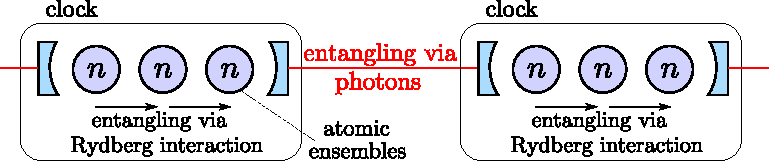
\includegraphics[width=0.45\textwidth]{./overview.pdf}
\caption
[Overview]
{
\label{fig:overview}
(Color online) Schematic of the setup. $K$ clocks, each holding $M$ atomic
ensembles of size $n$ are connected. Atoms within each ensemble get entangled
using long-range interaction between Rydberg atoms, ensembles in the same
clock are entangled  either via Rydberg interactions  or via the cavity
mode, while neighboring clocks are entangled through single-photon quantum channels,
enhanced by optical cavities.
The resulting state is a global GHZ state, $\ket{0}^{\otimes N} + \ket{1}^{\otimes
N}$ of all $N = KMn$ atoms in the network.}
\end{figure}

We imagine preparing all atoms in the ground state $g$, after which
our protocol consists of five subsequent steps.
First, using blockade, we create two independent collective excitations in one
ensemble in each clock, using two separate atomic levels ($f$ and $s$).
Second, each excited ensemble emits single photon pulses that are entangled with
one of these collective excitations.
Third, the photons are sent towards the neighboring atomic clocks, and measured
with a linear optics setup in Bell-basis. Fourth, upon success, each clock
performs a local CNOT operation to connect the two collective excitations. The
result is a set of $K$ entangled collective excitations, one in the first
ensemble of each clock, which serve as "seeds" for a global GHZ state.
In the fifth, and final, step the clocks locally "grow" a GHZ state out of each
seed, extending it to all atoms in the clock, and thus a global GHZ state is
obtained.
In the following, we provide detailed description and analysis of these five
steps, discuss the specific realization in Yb atoms and analyze the most
important sources of imperfections and errors.

Our scheme makes use of the Rydberg blockade, which is a result
of the interaction arising between atoms excited to Rydberg states in an
ensemble. If driven resonantly, the first excited atom blocks the transition of
a second one, thus at most one atom can get coherently excited to the Rydberg
state \cite{Dudin2012, Dudin2010, Ebert2015}, allowing precise quantum control.
Rydberg blockade has been proposed as an efficient tool to realize quantum gates
and perform quantum information processing \cite{Lukin2001, Muller2009,
Saffman2010, Zhao2010, Han2010, Goerz2014}. Efficient control requires the
atoms to reside within the blockade radius of the Rydberg atom.
Different ways of trapping and manipulating Rydberg states are currently  under
investigation both  experimentally \cite{Chen2010, Bariani2012, Firstenberg2013,
Antezza2014, Weber2015} and theoretically \cite{Topcu2013, Beterov2013,
Topcu2014}. 

%%%%%%%%%%%%%%%%%%%%%%%%%%%%%%%%%%%%%%%%%%%%%%%%%%%%%%%%%%%%%%%%%%%%%%%%%%%%%%%%%%5
% Collective excitations
%%%%%%%%%%%%%%%%%%%%%%%%%%%%%%%%%%%%%%%%%%%%%%%%%%%%%%%%%%%%%%%%%%%%%%%%%%%%%%%%%%5
In the first step, we make use of the Rydberg blockade to create a superposition
of one and zero excitation in both $f$ and $s$ levels, following the approach of
\cite{Lukin2001, Saffman2010,Dudin2012}.
This is done by performing the following sequence of driving pulses:
$[\pi/(2\sqrt{n})]_{g,r1}$, $[\pi]_{f,r1}$, $[\pi]_{f,s}$,
$[(\pi/(2\sqrt{n})]_{g,r1}$, $[\pi]_{f,r1}$, shown in \reffig{fig:steps123}(a),
where $[\phi]_{a,b}$ stands for a pulse with total, single-atom Rabi phase
$\phi$ between level $a$ and $b$.
Starting from the state $\ket{g}^{\otimes n} =: \ket{0}$, this pulse sequence
creates the state
\bel
\label{eq:step1}
(1 + f\+) (1 + s\+) \ket{0} =:
\Big(\ket{0_f} + \ket{1_f}\Big) \Big(\ket{0_s} + \ket{1_s}\Big), 
\eel 
where $f\+$
and $s\+$ are creation operators of the two (approximately) independent spin
wave modes, supported by the two levels $f$ and $s$. 

\begin{figure}
\centering
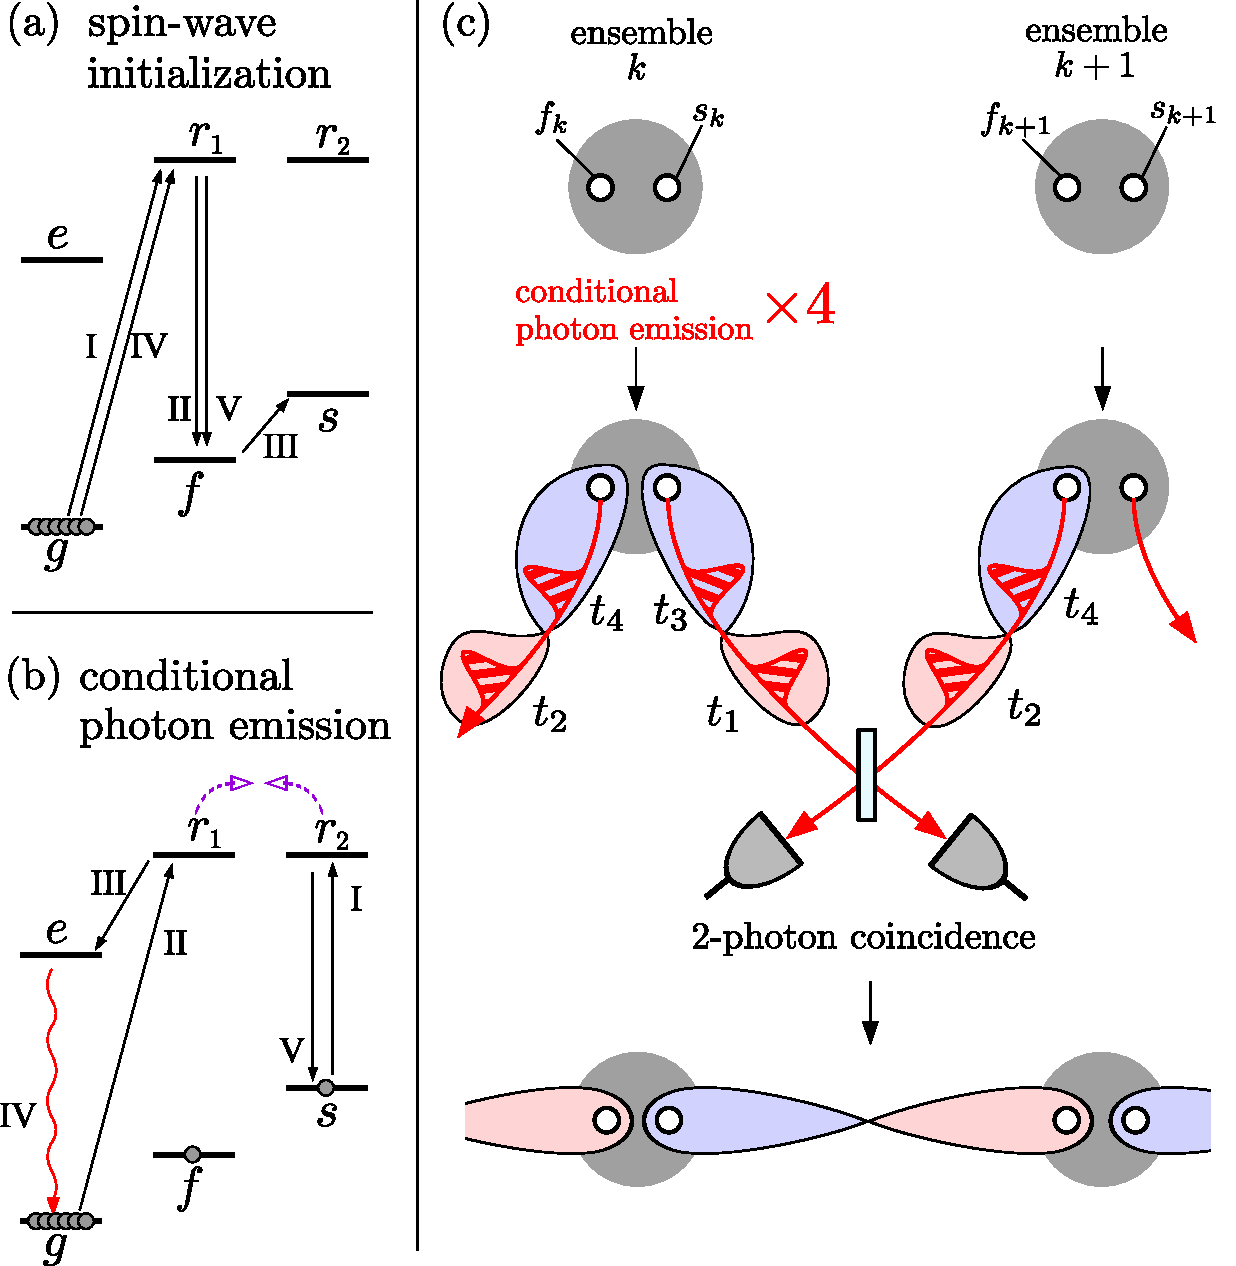
\includegraphics[width=0.45\textwidth]{./steps123.pdf}
\caption
[Steps to generate of pairwise entanglement]
{
\label{fig:steps123}
(Color online) Steps to generate pairwise entanglement. (a) Pulse
sequence used to initialize the spin-waves $f$ and $s$ in an ensemble.
(b) Pulse sequence inducing a conditional photon emission, the emitted photon
becomes entangled with the spin state $s$. 
(c) In three steps, neighboring ensembles generate pairwise entanglement between
their collective excitations. First, they induce $0+1$ superpositions of the two
independent spin waves, $f\+$ and $s\+$. Then applying the conditional photon
emission sequence four times, they emit four pulses, containing two
photons total. Each pair of photons is correlated with a unique spin state.
Finally, photons are measured with a linear optics setup, and 2-photon coincidences
indicate the creation of entanglement between neighboring ensembles. (Blue and
red shadings indicate positive and negative correlation between qubits,
respectively.)}
\end{figure}

%%%%%%%%%%%%%%%%%%%%%%%%%%%%%%%%%%%%%%%%%%%%%%%%%%%%%%%%%%%%%%%%%%%%%%%%%%%%%%%%%%5
% Photon emission
%%%%%%%%%%%%%%%%%%%%%%%%%%%%%%%%%%%%%%%%%%%%%%%%%%%%%%%%%%%%%%%%%%%%%%%%%%%%%%%%%%5
In the second step, spin-photon entangled states, using the spin wave modes $f$
and $s$, are created, based on an extended version of the scheme described
in \cite{Li2013} and collective enhancement. Each spin-photon entangled state is
created by the pulse sequence shown in \reffig{fig:steps123}(b), involving
$[\pi]_{s,r2}$, $[\pi/\sqrt{n}]_{g,r1}$, $[\pi]_{e,r1}$, $[\pi]_{s,r2}$. With additional pulses
applied before and after this sequence flipping between $0_f\leftrightarrow
1_f$, $0_s\leftrightarrow 1_s$ and swapping $f$ and $s$ waves, and proper
timing, this is repeated four times to produce four time-bin separated light
pulses, which are entangled with the two spin waves,
\bal
	&& \Big(
	\ket{0_f}\ket{t_2} + \ket{1_f}\ket{t_4}
	\Big)
	\Big(
	\ket{0_s}\ket{t_1} + \ket{1_s}\ket{t_3}
	\Big),
\label{eq:step2}
\eal
where $\ket{t_j}\ket{t_k}$ is a two photon state with photons emitted at times
$t_j$ and $t_k$.

%%%%%%%%%%%%%%%%%%%%%%%%%%%%%%%%%%%%%%%%%%%%%%%%%%%%%%%%%%%%%%%%%%%%%%%%%%%%%%%%%%5
% Photon detection
%%%%%%%%%%%%%%%%%%%%%%%%%%%%%%%%%%%%%%%%%%%%%%%%%%%%%%%%%%%%%%%%%%%%%%%%%%%%%%%%%%5
In the third step, pairs of time-bin encoded photon pulses from two neighboring
ensembles are detected by interfering the two pulses on a beam splitter and
measuring two-photon coincidences \cite{Duan2001, Honjo2007, Rubenok2013}.
As a result, entangled states between neighboring atomic ensembles, $k$ and
$k+1$, are created \cite{Lukin2003, Shwa2013},
\bel
	\ket{0_s}_k\ket{1_f}_{k+1} \pm \ket{1_s}_k \ket{0_f}_{k+1},
\eel
where the individual kets represent the states of $f$ and $s$ spin waves in the
two ensembles, see \reffig{fig:steps123}(c).


%%%%%%%%%%%%%%%%%%%%%%%%%%%%%%%%%%%%%%%%%%%%%%%%%%%%%%%%%%%%%%%%%%%%%%%%%%%%%%%%%%5
% Local connection
%%%%%%%%%%%%%%%%%%%%%%%%%%%%%%%%%%%%%%%%%%%%%%%%%%%%%%%%%%%%%%%%%%%%%%%%%%%%%%%%%%5
In the fourth step, the ensembles perform a local CNOT operation on the two
collective degrees of freedom, $f\+$ and $s\+$. This is done with the
following pulse sequence, $[\pi]_{s,r2}$, $[\pi]_{f,r1}$,
$[\pi/\sqrt{n}]_{g,r1}$, $[\pi]_{f,r1}$, $[\pi]_{s,r2}$, shown on
\reffig{fig:connection}(a). This promotes any population in $s$ to $r_2$,
which then blocks the path $g\leftrightarrow r_1 \leftrightarrow f$.
The result is a conditional flip $\ket{0_f} \leftrightarrow \ket{1_f}$,
conditioned on having zero $s\+$ excitations. If we perform $f\leftrightarrow s$
swaps before and after this process, we get a coherent flip between $\ket{0_f,
0_s} \leftrightarrow \ket{0_f, 1_s}$.

To understand the resulting state, let us consider two
entangled links, connecting three neighboring ensembles $k-1,k$ and
$k+1$ as shown in \reffig{fig:connection}(b). The corresponding state, before
the fourth step, is
\bel 
	\big(\ket{0_{s_{k-1}},1_{f_k}} + \ket{1_{s_{k-1}},0_{f_k}}\big)
	\otimes
	\big(\ket{0_{s_{k}},1_{f_{k+1}}} + \ket{1_{s_{k}},0_{f_{k+1}}}\big),
\eel
where $\ket{n_{s_{k-1}}, n_{f_k}}\otimes\ket{n_{s_k},n_{f_{k+1}}}$ indicate the
number of excitations in the modes $s_{k-1}, f_k, s_k, f_{k+1}$ of the three
ensembles.
After the conditional flip of $s_k$ and measurement of $n_{s_k}$, yielding $m
\in \{0,1\}$, the state becomes $\ket{0,1, 1-m} + \ket{1,0,m}$, where the
remaining kets stand for $\ket{n_{s_{k-1}}, n_{f_k}, n_{f_{k+1}}}$.
Depending on the outcome, either only $f_k$ (if $n_{s_k} = 1$) or the
entire right hand side (if $n_{s_k} = 0$) needs to be flipped in order
to obtain the desired GHZ state, $\bigotimes_k \ket{0_{f_k}} + \bigotimes_k
\ket{1_{f_k}}$, of the $f$ excitations of each clock, $k = 1,2,\dots K$.
\begin{figure}
\centering 
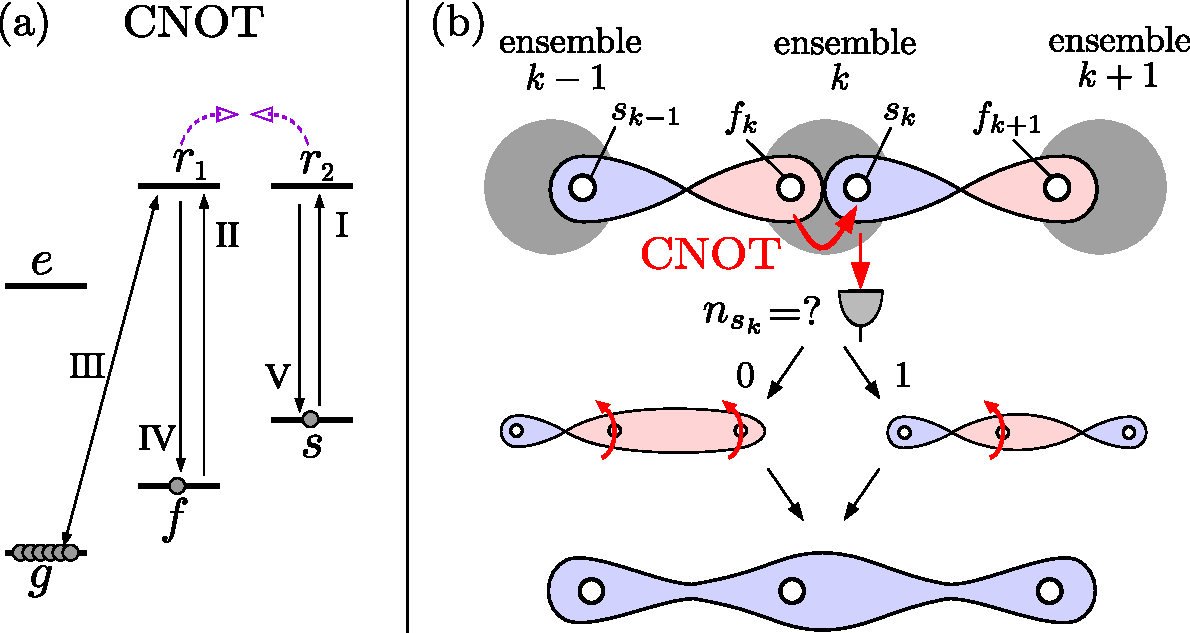
\includegraphics[width=0.45\textwidth]{./connection.pdf}
\caption
[Connecting links into non-local GHZ state]
{
\label{fig:connection} 
(Color online) Connecting links into non-local GHZ state.
(a) CNOT gate between
the two excitations $f$ and $s$: If level $s$ is occupied, then the coherent
(de)excitation of the $f$ level is blocked by the Rydberg blockade between
the $r_1$ and $r_2$ intermediate levels, otherwise it succeeds. 
(b) Connecting two entanglement links. The local CNOT and measurement
operations on ensemble $k$ entangle the two, initially independent, parts of
the system:
$s_{k-1}, f_k$ and $s_k, f_{k+1}$. Depending on the
outcome of the measurement, either only $f_k$, or the entire
right hand side needs to be flipped, in order to arrive to the proper GHZ
state.}
\end{figure} 


%%%%%%%%%%%%%%%%%%%%%%%%%%%%%%%%%%%%%%%%%%%%%%%%%%%%%%%%%%%%%%%%%%%%%%%%%%%%%%%%%%5
% Local GHZ growing
%%%%%%%%%%%%%%%%%%%%%%%%%%%%%%%%%%%%%%%%%%%%%%%%%%%%%%%%%%%%%%%%%%%%%%%%%%%%%%%%%%5
In the fifth step, each clock locally extends the entanglement from its $f$ degree
of freedom to all atoms using a collective Rydberg gate similar to the ones
introduced in Refs.
\cite{Saffman2009, Weimer2010}. In the case when each clock consists of a
single blockaded ensemble, the pulse sequence $[\pi]_{f,s}$, $[\pi/2]_{s,r2}$,
$\left([\pi/\sqrt{n-j+1}]_{g,r1}, [\pi/\sqrt{j}]_{f,r1}\;\text{for}\;
j=1,2,\dots n\right)$, $[\pi]_{s,r2}$, shown in \reffig{fig:GHZ}(a),  does
exactly that.
This sequence transfers the atoms one by one from $g$ to $f$ only if $r_2$ is
unoccupied, and gets blocked otherwise. The result is
\bel
\label{eq:step5}
	\bigotimes_{k=1}^{K}\ket{0_f}_k  + \bigotimes_{k=1}^{K}\ket{1_f}_k
	\;\rightarrow\; \bigotimes_{k=1}^K \ket{f}^{\otimes n} + \bigotimes_{k=1}^K
	s\+\ket{g}^{\otimes n},
\eel
where $\ket{f}$ and $\ket{g}$ denote the state of a single atom.
Finally, we get rid of
the $s$ excitation with a series of pulses that move it back to $g$:
$[\pi]_{f,s}$, $[\pi]_{f,r1}$, $[\pi]_{f,s}$, $[\pi/\sqrt{n}]_{g,r1}$, and end
up with $\ket{f}^{\otimes Kn} + \ket{g}^{\otimes Kn}$, a fully entangled state
of all $N = Kn$ atoms in the network. 
\begin{figure}
\centering
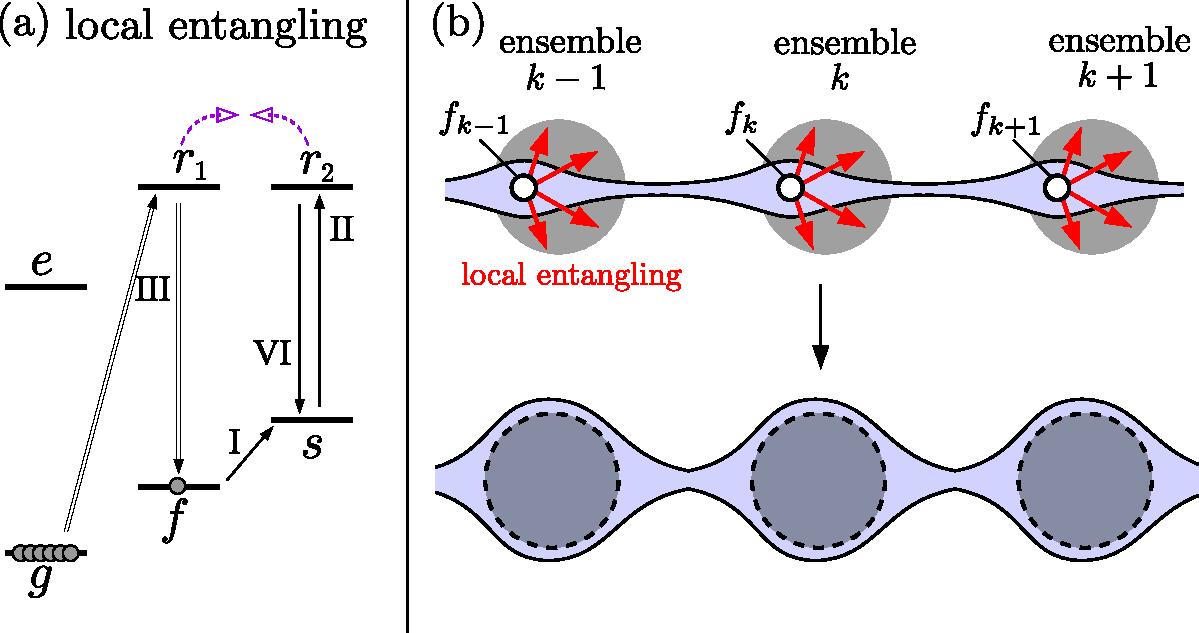
\includegraphics[width=0.45\textwidth]{./GHZ.pdf}
\caption
[Local GHZ creation]
{  
\label{fig:GHZ}
(Color online) Local GHZ creation.
(a) Conditional, local GHZ state generation: Any excitation in level $s$
prevents the transfer from $g$ to $f$. (b) The local entangling operation
extends the GHZ state from the $f$ spin-wave to all atoms. As a result, every
atom in the network gets entangled.}
\end{figure}

In practice, lattice clocks can employ $n = 10^3-10^4$ atoms each, that can not be manipulated simultaneously 
with high fidelity using Rydberg blockade (see discussion below).  In such a case,  the atoms can be separated into $M \sim 10$ ensembles
within each clock, as shown in Figure 1.  Efficient local entanglement
can be achieved with techniques described in \cite{Sorensen2000} or by using an
individually addressed ``messenger'' atom, that can be moved to the vicinity of
each ensemble to entangle all atoms within each clock using dipole-dipole
interaction. In such a case, the messenger atom can used, first, to extend the
entanglement to all ensembles in each clock, resulting in a state
$\ket{1_f}^{KM} + \ket{0}^{KM}$, after which the procedure shown in
\reffig{fig:GHZ}(a) applied within each ensemble can be used to a fully
entangled state of all $N = K \times Mn$ atoms in the network. (See
Supplementary for details.)





%%%%%%%%%%%%%%%%%%%%%%%%%%%%%%%%%%%%%%%%%%%%%%%%%%%%%%%%%%%%%%%%%%%%%%%%%%%%%%%%%%5
%%%%%%%%%%%%%%%%%%%%%%%%%%%%%%%%%%%%%%%%%%%%%%%%%%%%%%%%%%%%%%%%%%%%%%%%%%%%%%%%%%5
% Error analysis + Implementation
%%%%%%%%%%%%%%%%%%%%%%%%%%%%%%%%%%%%%%%%%%%%%%%%%%%%%%%%%%%%%%%%%%%%%%%%%%%%%%%%%%5
%%%%%%%%%%%%%%%%%%%%%%%%%%%%%%%%%%%%%%%%%%%%%%%%%%%%%%%%%%%%%%%%%%%%%%%%%%%%%%%%%%5
Next, we investigate  the robustness of our  protocol  in  light of realistic
physical imperfections.
We assume that all imperfections decrease the coherence between the two
components of the GHZ state, and therefore the fidelity can be written as
$F = [1 + \exp(-\eps_\text{tot})]/2$, where $\eps_\text{tot}$ is the sum of the
errors.
The errors arising during each non-local connection step
$\eps_\text{non-local}$ and the errors arising during a local GHZ creation
in one clock $\eps_\text{local}$ add up to the total error 
\bel
	\eps_\text{tot} = (K-1)\eps_\text{non-local} + KM\eps_\text{local}.
\eel
This error increases linearly with the total number of atoms in the network,
$N$, and the coefficient, $(\eps_\text{non-local}/M + \eps_\text{local})/n$,
depends on the number of atoms, $n$, within a single atom cloud under blockade.
For a certain optimal local atom number $n_\text{opt}$, the total fidelity is
maximal, i.e. decreases with the slowest rate, as $N$ increases.


To be specific, we focus on a possible implementation of our scheme with
ensembles of neutral ytterbium atoms whose relevant electronic levels are shown on
\reffig{fig:Yb_levels}.
\begin{figure}[h]
\centering
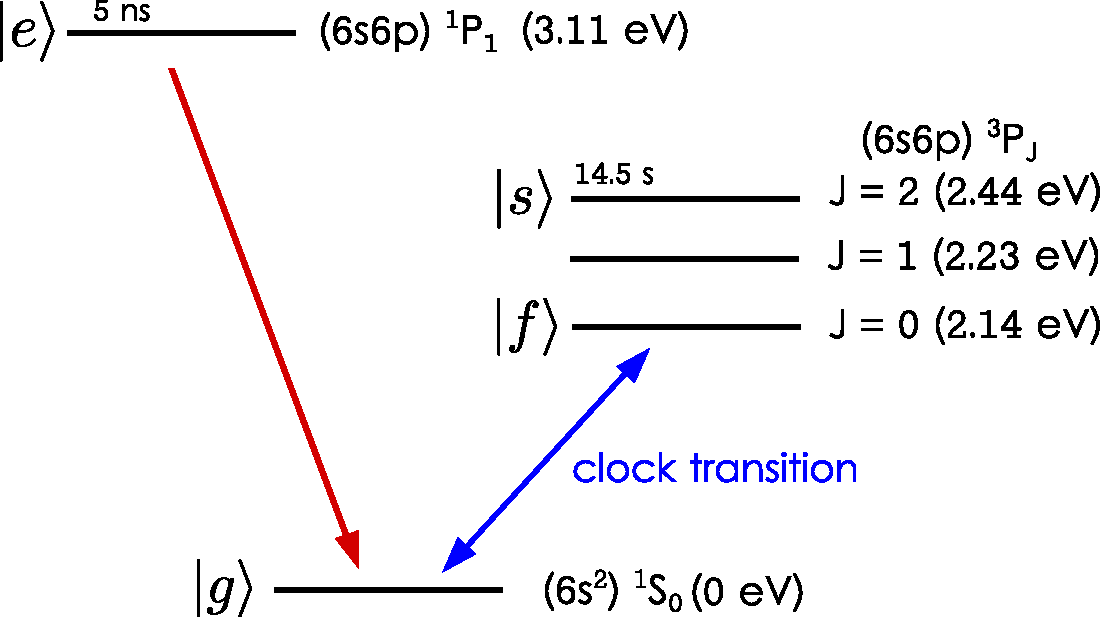
\includegraphics[width=0.45\textwidth]{./Yb_levels.pdf}
\caption
[Implementation with Yb levels]
{ 
\label{fig:Yb_levels}
(Color online)
Implementation of our protocol in the lower level of neutral Yb. We assign
the roles of $g$ and $f$ to the clock levels, the role of $s$ to the metastable
$J=2$ level of $6s6p$, and the role of $e$ to the ${}^1P_1$  excited
state, which spontaneously decays to the ground state.}
\end{figure}
We identify the  following levels of neutral
Yb  relevant for our protocol:
$\ket{g} = \ket{6s^2({}^1\!S_0)}$, 
$\ket{f} = \ket{6s6p({}^3\!P_0)}$, 
$\ket{s} = \ket{6s6p({}^3\!P_2)}$ and 
$\ket{e} = \ket{6s6p({}^1\!P_1)}$, and 
two Rydberg levels 
$\ket{r_1} = \ket{6s\tilde n p_{m=+1}({}^1P_1)}$ and 
$\ket{r_2} = \ket{6s\tilde n s({}^3S_1)}$ 
with the same principle quantum number $\tilde n$. 
Collective enhancement and phase matching of the laser pulses make the emitted
photons leave in a well-defined, narrow solid angle, resulting in high photon
collection efficiency.
Due to the different symmetries of these
states, the coherent coupling can be done via 1-photon transitions for
$r_1\leftrightarrow g$ and $r_2\leftrightarrow s$, and requires 2-photon
transitions for $r_1\leftrightarrow e$ and $r_1\leftrightarrow f$. 
We envision the atoms
being held in position by an optical lattice with period $a =
275.75~\text{nm}$, each potential minimum holding exactly one Yb atom.
(The lattice intensity can be modulated during the Rydberg state excitation
\cite{Tiecke2014}.)  Overall fidelity turns out to depend on the
lattice geometry; it is the highest for 3D optical lattice.
  
We consider the following errors in our analysis. During
non-local connection, we take into account the finite $r_1$-$r_2$ interaction, which
allows the creation of an $r_1$ excitation with some small probability, even if
$r_2$ is populated, the finite lifetime of the $s$ and $r_2$ levels,
and
the dark-count rate of photo-detectors. For the local GHZ creation step, we account
for the same imperfection of the
$r_1$-$r_2$ blockade as for the non-local entangling step, the finite lifetimes
of the Rydberg levels $r_1$ and $r_2$, and the imperfect self-blockade of the
single excited Rydberg states $r_1$.
(See Supplementary Materials for details.) We estimate the effect of these
errors, and numerically optimize the free parameters: the Rabi frequency
$\Omega$ of the transferring pulses $g\rightarrow r_1$ and $r_1\rightarrow f$,
and the number of local atoms $n$, for principle quantum numbers, $50\leq \tilde
n \leq 150$ of the Rydberg levels, in order to find the minimal error per atom,
$E := \eps_\text{tot}/N$. 
 
To illustrate, for Rydberg levels $\tilde n = 120$, we find that the highest
fidelity is reached for $n_\text{opt} \approx 146$, and $\Omega = 10^5\,\gamma$,
where $\gamma \sim 10^3\,\text{s}^{-1}$ is the natural linewidth of the Rydberg
levels, for a clock size of $(Mn)_\text{opt} = 2500$. In this case, the error
per atom is $E_\text{min}= [\eps_\text{tot}/N]_\text{min} = 1.8 \times 10^{-5}$.
Contributions of the different error sources are shown in Table
\ref{table:errors}. We find that the decay of the Rydberg level, and imperfect
blockade cause the majority of imperfections, both arising during the critical
step, local extension of the GHZ state. (See Supplementary Materials for more
details.)
\begin{table}
\centering
\begin{tabular}{|l|c|c|}
\hline
 Errors in 3D ensemble & error per atom & ratio in total\\
\hline
imperfect blockade ($e_1$) 	& $2.6 \times 10^{-6}$ 	& 14\%\\
Rydberg decay ($e_2$) 		& $1.6 \times 10^{-5}$ 	& 86\%\\
self-blockade ($e_3$) 		& $\sim 10^{-11}$ 	& $<0.1$\%\\
$r_2$ decay (non-local) ($e_4$) & $ \sim 10^{-11}$ 	& $<0.1$\%\\
photon detection ($e_5$) 	& $ \sim 10^{-12}$ 		& $<0.1$\%\\
memory error ($e_6$) 		& $ \sim 10^{-8}$ 	& $<0.1$\%\\
photon collection ($e_7$) & $\sim 10^{-8}$ & $<0.1$\%\\
\hline
total error per atom 		& $1.8 \times 10^{-5}$ 	& 100\%\\
\hline
\end{tabular}
\caption
[Error budget]{
\label{table:errors}
The absolute and relative contribution of the different error sources to the
total error per atom $E$, at $\tilde n = 120$, $\Omega = \Omega_\text{opt} = 
10^5\,\gamma$ and $n = n_\text{opt} = 146$, after numerical
optimization, for a 3D lattice.
(See Supplementary Materials for 2D results.)}
\end{table}

%%%%%%%%%%%%%%%%%%%%%%%%%%%%%%%%%%%%%%%%%%%%%%%%%%%%%%%%%%%%%%%%%%%%%%%%%%%%%%%%%%5
%%%%%%%%%%%%%%%%%%%%%%%%%%%%%%%%%%%%%%%%%%%%%%%%%%%%%%%%%%%%%%%%%%%%%%%%%%%%%%%%%%5
% Clock network optimization
%%%%%%%%%%%%%%%%%%%%%%%%%%%%%%%%%%%%%%%%%%%%%%%%%%%%%%%%%%%%%%%%%%%%%%%%%%%%%%%%%%5
%%%%%%%%%%%%%%%%%%%%%%%%%%%%%%%%%%%%%%%%%%%%%%%%%%%%%%%%%%%%%%%%%%%%%%%%%%%%%%%%%%5
With the optimal ensemble size $n_\text{opt}$, determined above, we consider the
total number of entangled atoms $N$. Although having more atoms always results
in improved clock precision, entangling all available atoms is not necessarily
optimal. To see this, we compare the stability of the entangled clock network
and a non-entangled network, and find an optimal entangled atom number
$N_\text{opt}$ by maximizing the stability gain over the non-entangled scheme,
\bel
\label{eq:gain}
	G = \frac{\sigma_\text{non-ent}}{\sigma_\text{ent}/(2F-1)} =
	e^{-EN}\frac{\pi}{8}\sqrt{\frac{N}{\log N}},
\eel 
where $\sigma_\text{ent} = \frac{1}{\omega_0 \tau}\frac{8}{\pi}\frac{\sqrt{\log
N}}{N}$ (from \cite{Komar2014}, assuming perfect fidelity, and that $\tau$ is
smaller than the reduced atomic coherence time $\gamma_\text{at}^{-1}/N$) and
$\sigma_\text{non-ent} = \frac{1}{\omega_0\tau}\frac{1}{\sqrt{N}}$ (for $N$
independent atoms) are the Allan deviations of the two schemes, where $\omega_0$
is the central frequency and $\tau$ is the total available measurement time.
The additional factor of $2F-1 = e^{-EN}$ is due to the reduced Fisher
information of a non-pure GHZ state, where $F$
is the fidelity of the initial state.
(See supplementary materials for details.) For $E = E_\text{min} = 1.8\times
10^{-5}$, \refeq{eq:gain} is maximized with optimal atom number $N_\text{opt}
\approx 1/(2E_\text{min}) \approx 25000$, where $G_\text{max} \sim 12$, and $F
= [1+e^{-N_\text{opt} E_\text{min}}]/2 = 0.82$. The optimal gain  is achieved by
25000 entangled atoms distributed in $K_\text{opt} = N_\text{opt}/(Mn)_\text{opt}
\approx 10$ clocks.



%%%%%%%%%%%%%%%%%%%%%%%%%%%%%%%%%%%%%%%%%%%%%%%%%%%%%%%%%%%%%%%%%%%%%%%%%%%%%%%%%%5
%%%%%%%%%%%%%%%%%%%%%%%%%%%%%%%%%%%%%%%%%%%%%%%%%%%%%%%%%%%%%%%%%%%%%%%%%%%%%%%%%%5
% Conclusion
%%%%%%%%%%%%%%%%%%%%%%%%%%%%%%%%%%%%%%%%%%%%%%%%%%%%%%%%%%%%%%%%%%%%%%%%%%%%%%%%%%5
%%%%%%%%%%%%%%%%%%%%%%%%%%%%%%%%%%%%%%%%%%%%%%%%%%%%%%%%%%%%%%%%%%%%%%%%%%%%%%%%%%5

We presented and analyzed a protocol, capable of fully entangling ensembles of
neutral atoms located in different atomic clocks. Local interactions are made
robust by utilizing the strong interaction between Rydberg excitations, and
non-local entanglement creation is made reliable with strong atom-light
coupling, suppressed photon propagation errors and long atomic memory lifetimes.
We showed that our scheme, in particular a realization with neutral Yb
ensembles, is feasible and provides significant gain over non-entangled schemes
even in the light of physical imperfections. Our results provide the first
detailed proposal for a neutral atom clock network that can serve as a first
prototype of the global quantum clock network outlined in \cite{Komar2014}.



%%%%%%%%%%%%%%%%%%%%%%%%%%%%%%%%%%%%%%%%%%%%%%%%%%%%%%%%%%%%%%%%%%%%%%%%%%%%%%%%%%5
%%%%%%%%%%%%%%%%%%%%%%%%%%%%%%%%%%%%%%%%%%%%%%%%%%%%%%%%%%%%%%%%%%%%%%%%%%%%%%%%%%5
% Acknowledgment
%%%%%%%%%%%%%%%%%%%%%%%%%%%%%%%%%%%%%%%%%%%%%%%%%%%%%%%%%%%%%%%%%%%%%%%%%%%%%%%%%%5
%%%%%%%%%%%%%%%%%%%%%%%%%%%%%%%%%%%%%%%%%%%%%%%%%%%%%%%%%%%%%%%%%%%%%%%%%%%%%%%%%%5

\begin{acknowledgements}
We are grateful to Kyle Beloy, Shimon Kolkowitz, Ronen Kroeze, Travis Nicholson,
Thibault Peyronel, Alp Sipahigil, Jeff Thompson, and Leo Zhou for enlightening
discussions.
This work was supported by NSF, CUA, NIST, NASA, Simons Foundation, AFOSR MURI,
ARL and NSSEFF fellowship.
\end{acknowledgements}

%\bibliography{Rydberg_GHZ}

%merlin.mbs apsrev4-1.bst 2010-07-25 4.21a (PWD, AO, DPC) hacked
%Control: key (0)
%Control: author (8) initials jnrlst
%Control: editor formatted (1) identically to author
%Control: production of article title (-1) disabled
%Control: page (0) single
%Control: year (1) truncated
%Control: production of eprint (0) enabled
\begin{thebibliography}{39}%
\makeatletter
\providecommand \@ifxundefined [1]{%
 \@ifx{#1\undefined}
}%
\providecommand \@ifnum [1]{%
 \ifnum #1\expandafter \@firstoftwo
 \else \expandafter \@secondoftwo
 \fi
}%
\providecommand \@ifx [1]{%
 \ifx #1\expandafter \@firstoftwo
 \else \expandafter \@secondoftwo
 \fi
}%
\providecommand \natexlab [1]{#1}%
\providecommand \enquote  [1]{``#1''}%
\providecommand \bibnamefont  [1]{#1}%
\providecommand \bibfnamefont [1]{#1}%
\providecommand \citenamefont [1]{#1}%
\providecommand \href@noop [0]{\@secondoftwo}%
\providecommand \href [0]{\begingroup \@sanitize@url \@href}%
\providecommand \@href[1]{\@@startlink{#1}\@@href}%
\providecommand \@@href[1]{\endgroup#1\@@endlink}%
\providecommand \@sanitize@url [0]{\catcode `\\12\catcode `\$12\catcode
  `\&12\catcode `\#12\catcode `\^12\catcode `\_12\catcode `\%12\relax}%
\providecommand \@@startlink[1]{}%
\providecommand \@@endlink[0]{}%
\providecommand \url  [0]{\begingroup\@sanitize@url \@url }%
\providecommand \@url [1]{\endgroup\@href {#1}{\urlprefix }}%
\providecommand \urlprefix  [0]{URL }%
\providecommand \Eprint [0]{\href }%
\providecommand \doibase [0]{http://dx.doi.org/}%
\providecommand \selectlanguage [0]{\@gobble}%
\providecommand \bibinfo  [0]{\@secondoftwo}%
\providecommand \bibfield  [0]{\@secondoftwo}%
\providecommand \translation [1]{[#1]}%
\providecommand \BibitemOpen [0]{}%
\providecommand \bibitemStop [0]{}%
\providecommand \bibitemNoStop [0]{.\EOS\space}%
\providecommand \EOS [0]{\spacefactor3000\relax}%
\providecommand \BibitemShut  [1]{\csname bibitem#1\endcsname}%
\let\auto@bib@innerbib\@empty
%</preamble>
\bibitem [{\citenamefont {Ludlow}\ and\ \citenamefont {Ye}(2015)}]{Ludlow2015}%
  \BibitemOpen
  \bibfield  {author} {\bibinfo {author} {\bibfnamefont {A.~D.}\ \bibnamefont
  {Ludlow}}\ and\ \bibinfo {author} {\bibfnamefont {J.}~\bibnamefont {Ye}},\
  }\href {\doibase http://dx.doi.org/10.1016/j.crhy.2015.03.008} {\bibfield
  {journal} {\bibinfo  {journal} {Comptes Rendus Physique}\ }\textbf {\bibinfo
  {volume} {16}},\ \bibinfo {pages} {499 } (\bibinfo {year}
  {2015})}\BibitemShut {NoStop}%
\bibitem [{\citenamefont {Hinkley}\ \emph {et~al.}(2013)\citenamefont
  {Hinkley}, \citenamefont {Sherman}, \citenamefont {Phillips}, \citenamefont
  {Schioppo}, \citenamefont {Lemke}, \citenamefont {Beloy}, \citenamefont
  {Pizzocaro}, \citenamefont {Oates},\ and\ \citenamefont
  {Ludlow}}]{Hinkley2013}%
  \BibitemOpen
  \bibfield  {author} {\bibinfo {author} {\bibfnamefont {N.}~\bibnamefont
  {Hinkley}}, \bibinfo {author} {\bibfnamefont {J.~A.}\ \bibnamefont
  {Sherman}}, \bibinfo {author} {\bibfnamefont {N.~B.}\ \bibnamefont
  {Phillips}}, \bibinfo {author} {\bibfnamefont {M.}~\bibnamefont {Schioppo}},
  \bibinfo {author} {\bibfnamefont {N.~D.}\ \bibnamefont {Lemke}}, \bibinfo
  {author} {\bibfnamefont {K.}~\bibnamefont {Beloy}}, \bibinfo {author}
  {\bibfnamefont {M.}~\bibnamefont {Pizzocaro}}, \bibinfo {author}
  {\bibfnamefont {C.~W.}\ \bibnamefont {Oates}}, \ and\ \bibinfo {author}
  {\bibfnamefont {A.~D.}\ \bibnamefont {Ludlow}},\ }\href {\doibase
  10.1126/science.1240420} {\bibfield  {journal} {\bibinfo  {journal}
  {Science}\ }\textbf {\bibinfo {volume} {341}},\ \bibinfo {pages} {1215}
  (\bibinfo {year} {2013})}\BibitemShut {NoStop}%
\bibitem [{\citenamefont {Bloom}\ \emph {et~al.}(2014)\citenamefont {Bloom},
  \citenamefont {Nicholson}, \citenamefont {Williams}, \citenamefont
  {Campbell}, \citenamefont {Bishof}, \citenamefont {Zhang}, \citenamefont
  {Zhang}, \citenamefont {Bromley},\ and\ \citenamefont {Ye}}]{Bloom2014}%
  \BibitemOpen
  \bibfield  {author} {\bibinfo {author} {\bibfnamefont {B.~J.}\ \bibnamefont
  {Bloom}}, \bibinfo {author} {\bibfnamefont {T.~L.}\ \bibnamefont
  {Nicholson}}, \bibinfo {author} {\bibfnamefont {J.~R.}\ \bibnamefont
  {Williams}}, \bibinfo {author} {\bibfnamefont {S.~L.}\ \bibnamefont
  {Campbell}}, \bibinfo {author} {\bibfnamefont {M.}~\bibnamefont {Bishof}},
  \bibinfo {author} {\bibfnamefont {X.}~\bibnamefont {Zhang}}, \bibinfo
  {author} {\bibfnamefont {W.}~\bibnamefont {Zhang}}, \bibinfo {author}
  {\bibfnamefont {S.~L.}\ \bibnamefont {Bromley}}, \ and\ \bibinfo {author}
  {\bibfnamefont {J.}~\bibnamefont {Ye}},\ }\href {\doibase
  10.1038/nature12941} {\bibfield  {journal} {\bibinfo  {journal} {Nature}\
  }\textbf {\bibinfo {volume} {506}},\ \bibinfo {pages} {71} (\bibinfo {year}
  {2014})}\BibitemShut {NoStop}%
\bibitem [{\citenamefont {Nicholson}\ \emph {et~al.}(2015)\citenamefont
  {Nicholson}, \citenamefont {Campbell}, \citenamefont {Hutson}, \citenamefont
  {Marti}, \citenamefont {Bloom}, \citenamefont {McNally}, \citenamefont
  {Zhang}, \citenamefont {Barrett}, \citenamefont {Safronova}, \citenamefont
  {Strouse}, \citenamefont {Tew},\ and\ \citenamefont {Ye}}]{Nicholson2015}%
  \BibitemOpen
  \bibfield  {author} {\bibinfo {author} {\bibfnamefont {T.}~\bibnamefont
  {Nicholson}}, \bibinfo {author} {\bibfnamefont {S.}~\bibnamefont {Campbell}},
  \bibinfo {author} {\bibfnamefont {R.}~\bibnamefont {Hutson}}, \bibinfo
  {author} {\bibfnamefont {G.}~\bibnamefont {Marti}}, \bibinfo {author}
  {\bibfnamefont {B.}~\bibnamefont {Bloom}}, \bibinfo {author} {\bibfnamefont
  {R.}~\bibnamefont {McNally}}, \bibinfo {author} {\bibfnamefont
  {W.}~\bibnamefont {Zhang}}, \bibinfo {author} {\bibfnamefont
  {M.}~\bibnamefont {Barrett}}, \bibinfo {author} {\bibfnamefont
  {M.}~\bibnamefont {Safronova}}, \bibinfo {author} {\bibfnamefont
  {G.}~\bibnamefont {Strouse}}, \bibinfo {author} {\bibfnamefont
  {W.}~\bibnamefont {Tew}}, \ and\ \bibinfo {author} {\bibfnamefont
  {J.}~\bibnamefont {Ye}},\ }\href {\doibase 10.1038/ncomms7896} {\bibfield
  {journal} {\bibinfo  {journal} {Nature Communications}\ }\textbf {\bibinfo
  {volume} {6}},\ \bibinfo {pages} {6896} (\bibinfo {year} {2015})}\BibitemShut
  {NoStop}%
\bibitem [{\citenamefont {Derevianko}\ and\ \citenamefont
  {Pospelov}(2014)}]{Derevianko_Nat_2014}%
  \BibitemOpen
  \bibfield  {author} {\bibinfo {author} {\bibfnamefont {A.}~\bibnamefont
  {Derevianko}}\ and\ \bibinfo {author} {\bibfnamefont {M.}~\bibnamefont
  {Pospelov}},\ }\href {\doibase 10.1038/nphys3137} {\bibfield  {journal}
  {\bibinfo  {journal} {Nature Physics}\ }\textbf {\bibinfo {volume} {10}},\
  \bibinfo {pages} {933} (\bibinfo {year} {2014})}\BibitemShut {NoStop}%
\bibitem [{\citenamefont {K\'{o}m\'{a}r}\ \emph {et~al.}(2014)\citenamefont
  {K\'{o}m\'{a}r}, \citenamefont {Kessler}, \citenamefont {Bishof},
  \citenamefont {Jiang}, \citenamefont {S{\o}rensen}, \citenamefont {Ye},\ and\
  \citenamefont {Lukin}}]{Komar2014}%
  \BibitemOpen
  \bibfield  {author} {\bibinfo {author} {\bibfnamefont {P.}~\bibnamefont
  {K\'{o}m\'{a}r}}, \bibinfo {author} {\bibfnamefont {E.~M.}\ \bibnamefont
  {Kessler}}, \bibinfo {author} {\bibfnamefont {M.}~\bibnamefont {Bishof}},
  \bibinfo {author} {\bibfnamefont {L.}~\bibnamefont {Jiang}}, \bibinfo
  {author} {\bibfnamefont {A.~S.}\ \bibnamefont {S{\o}rensen}}, \bibinfo
  {author} {\bibfnamefont {J.}~\bibnamefont {Ye}}, \ and\ \bibinfo {author}
  {\bibfnamefont {M.~D.}\ \bibnamefont {Lukin}},\ }\href {\doibase
  10.1038/nphys3000} {\bibfield  {journal} {\bibinfo  {journal} {Nature
  Physics}\ }\textbf {\bibinfo {volume} {10}},\ \bibinfo {pages} {582}
  (\bibinfo {year} {2014})}\BibitemShut {NoStop}%
\bibitem [{\citenamefont {Kessler}\ \emph {et~al.}(2014)\citenamefont
  {Kessler}, \citenamefont {K\'{o}m\'{a}r}, \citenamefont {Bishof},
  \citenamefont {Jiang}, \citenamefont {S{\o}rensen}, \citenamefont {Ye},\ and\
  \citenamefont {Lukin}}]{Kessler2014}%
  \BibitemOpen
  \bibfield  {author} {\bibinfo {author} {\bibfnamefont {E.~M.}\ \bibnamefont
  {Kessler}}, \bibinfo {author} {\bibfnamefont {P.}~\bibnamefont
  {K\'{o}m\'{a}r}}, \bibinfo {author} {\bibfnamefont {M.}~\bibnamefont
  {Bishof}}, \bibinfo {author} {\bibfnamefont {L.}~\bibnamefont {Jiang}},
  \bibinfo {author} {\bibfnamefont {A.~S.}\ \bibnamefont {S{\o}rensen}},
  \bibinfo {author} {\bibfnamefont {J.}~\bibnamefont {Ye}}, \ and\ \bibinfo
  {author} {\bibfnamefont {M.~D.}\ \bibnamefont {Lukin}},\ }\href {\doibase
  10.1103/PhysRevLett.112.190403} {\bibfield  {journal} {\bibinfo  {journal}
  {Phys. Rev. Lett.}\ }\textbf {\bibinfo {volume} {112}},\ \bibinfo {pages}
  {190403} (\bibinfo {year} {2014})}\BibitemShut {NoStop}%
\bibitem [{\citenamefont {Berry}\ \emph {et~al.}(2009)\citenamefont {Berry},
  \citenamefont {Higgins}, \citenamefont {Bartlett}, \citenamefont {Mitchell},
  \citenamefont {Pryde},\ and\ \citenamefont {Wiseman}}]{Berry2009}%
  \BibitemOpen
  \bibfield  {author} {\bibinfo {author} {\bibfnamefont {D.~W.}\ \bibnamefont
  {Berry}}, \bibinfo {author} {\bibfnamefont {B.~L.}\ \bibnamefont {Higgins}},
  \bibinfo {author} {\bibfnamefont {S.~D.}\ \bibnamefont {Bartlett}}, \bibinfo
  {author} {\bibfnamefont {M.~W.}\ \bibnamefont {Mitchell}}, \bibinfo {author}
  {\bibfnamefont {G.~J.}\ \bibnamefont {Pryde}}, \ and\ \bibinfo {author}
  {\bibfnamefont {H.~M.}\ \bibnamefont {Wiseman}},\ }\href {\doibase
  10.1103/PhysRevA.80.052114} {\bibfield  {journal} {\bibinfo  {journal} {Phys.
  Rev. A}\ }\textbf {\bibinfo {volume} {80}},\ \bibinfo {pages} {052114}
  (\bibinfo {year} {2009})}\BibitemShut {NoStop}%
\bibitem [{\citenamefont {Hall}\ \emph {et~al.}(2012)\citenamefont {Hall},
  \citenamefont {Berry}, \citenamefont {Zwierz},\ and\ \citenamefont
  {Wiseman}}]{Hall2012}%
  \BibitemOpen
  \bibfield  {author} {\bibinfo {author} {\bibfnamefont {M.~J.~W.}\
  \bibnamefont {Hall}}, \bibinfo {author} {\bibfnamefont {D.~W.}\ \bibnamefont
  {Berry}}, \bibinfo {author} {\bibfnamefont {M.}~\bibnamefont {Zwierz}}, \
  and\ \bibinfo {author} {\bibfnamefont {H.~M.}\ \bibnamefont {Wiseman}},\
  }\href {\doibase 10.1103/PhysRevA.85.041802} {\bibfield  {journal} {\bibinfo
  {journal} {Phys. Rev. A}\ }\textbf {\bibinfo {volume} {85}},\ \bibinfo
  {pages} {041802} (\bibinfo {year} {2012})}\BibitemShut {NoStop}%
\bibitem [{\citenamefont {Hosten}\ \emph {et~al.}(2016)\citenamefont {Hosten},
  \citenamefont {Engelsen}, \citenamefont {Krishnakumar},\ and\ \citenamefont
  {Kasevich}}]{Hosten2016}%
  \BibitemOpen
  \bibfield  {author} {\bibinfo {author} {\bibfnamefont {O.}~\bibnamefont
  {Hosten}}, \bibinfo {author} {\bibfnamefont {N.~J.}\ \bibnamefont
  {Engelsen}}, \bibinfo {author} {\bibfnamefont {R.}~\bibnamefont
  {Krishnakumar}}, \ and\ \bibinfo {author} {\bibfnamefont {M.~A.}\
  \bibnamefont {Kasevich}},\ }\href {\doibase 10.1038/nature16176} {\bibfield
  {journal} {\bibinfo  {journal} {Nature}\ }\textbf {\bibinfo {volume} {529}},\
  \bibinfo {pages} {505} (\bibinfo {year} {2016})}\BibitemShut {NoStop}%
\bibitem [{\citenamefont {Sangouard}\ \emph {et~al.}(2011)\citenamefont
  {Sangouard}, \citenamefont {Simon}, \citenamefont {de~Riedmatten},\ and\
  \citenamefont {Gisin}}]{Sangouard2011}%
  \BibitemOpen
  \bibfield  {author} {\bibinfo {author} {\bibfnamefont {N.}~\bibnamefont
  {Sangouard}}, \bibinfo {author} {\bibfnamefont {C.}~\bibnamefont {Simon}},
  \bibinfo {author} {\bibfnamefont {H.}~\bibnamefont {de~Riedmatten}}, \ and\
  \bibinfo {author} {\bibfnamefont {N.}~\bibnamefont {Gisin}},\ }\href
  {\doibase 10.1103/RevModPhys.83.33} {\bibfield  {journal} {\bibinfo
  {journal} {Rev. Mod. Phys.}\ }\textbf {\bibinfo {volume} {83}},\ \bibinfo
  {pages} {33} (\bibinfo {year} {2011})}\BibitemShut {NoStop}%
\bibitem [{\citenamefont {S{\o}rensen}\ and\ \citenamefont
  {M{\o}lmer}(1999)}]{Sorensen1999}%
  \BibitemOpen
  \bibfield  {author} {\bibinfo {author} {\bibfnamefont {A.}~\bibnamefont
  {S{\o}rensen}}\ and\ \bibinfo {author} {\bibfnamefont {K.}~\bibnamefont
  {M{\o}lmer}},\ }\href {\doibase 10.1103/PhysRevLett.82.1971} {\bibfield
  {journal} {\bibinfo  {journal} {Phys. Rev. Lett.}\ }\textbf {\bibinfo
  {volume} {82}},\ \bibinfo {pages} {1971} (\bibinfo {year}
  {1999})}\BibitemShut {NoStop}%
\bibitem [{\citenamefont {Saffman}\ \emph {et~al.}(2010)\citenamefont
  {Saffman}, \citenamefont {Walker},\ and\ \citenamefont
  {M{\o}lmer}}]{Saffman2010}%
  \BibitemOpen
  \bibfield  {author} {\bibinfo {author} {\bibfnamefont {M.}~\bibnamefont
  {Saffman}}, \bibinfo {author} {\bibfnamefont {T.~G.}\ \bibnamefont {Walker}},
  \ and\ \bibinfo {author} {\bibfnamefont {K.}~\bibnamefont {M{\o}lmer}},\
  }\href {\doibase 10.1103/RevModPhys.82.2313} {\bibfield  {journal} {\bibinfo
  {journal} {Rev. Mod. Phys.}\ }\textbf {\bibinfo {volume} {82}},\ \bibinfo
  {pages} {2313} (\bibinfo {year} {2010})}\BibitemShut {NoStop}%
\bibitem [{\citenamefont {Dudin}\ and\ \citenamefont
  {Kuzmich}(2012)}]{Dudin2012}%
  \BibitemOpen
  \bibfield  {author} {\bibinfo {author} {\bibfnamefont {Y.~O.}\ \bibnamefont
  {Dudin}}\ and\ \bibinfo {author} {\bibfnamefont {A.}~\bibnamefont
  {Kuzmich}},\ }\href {\doibase 10.1126/science.1217901} {\bibfield  {journal}
  {\bibinfo  {journal} {Science}\ }\textbf {\bibinfo {volume} {336}},\ \bibinfo
  {pages} {887} (\bibinfo {year} {2012})}\BibitemShut {NoStop}%
\bibitem [{\citenamefont {Dudin}\ \emph {et~al.}(2010)\citenamefont {Dudin},
  \citenamefont {Radnaev}, \citenamefont {Zhao}, \citenamefont {Blumoff},
  \citenamefont {Kennedy},\ and\ \citenamefont {Kuzmich}}]{Dudin2010}%
  \BibitemOpen
  \bibfield  {author} {\bibinfo {author} {\bibfnamefont {Y.~O.}\ \bibnamefont
  {Dudin}}, \bibinfo {author} {\bibfnamefont {A.~G.}\ \bibnamefont {Radnaev}},
  \bibinfo {author} {\bibfnamefont {R.}~\bibnamefont {Zhao}}, \bibinfo {author}
  {\bibfnamefont {J.~Z.}\ \bibnamefont {Blumoff}}, \bibinfo {author}
  {\bibfnamefont {T.~A.~B.}\ \bibnamefont {Kennedy}}, \ and\ \bibinfo {author}
  {\bibfnamefont {A.}~\bibnamefont {Kuzmich}},\ }\href {\doibase
  10.1103/PhysRevLett.105.260502} {\bibfield  {journal} {\bibinfo  {journal}
  {Phys. Rev. Lett.}\ }\textbf {\bibinfo {volume} {105}},\ \bibinfo {pages}
  {260502} (\bibinfo {year} {2010})}\BibitemShut {NoStop}%
\bibitem [{\citenamefont {Ebert}\ \emph {et~al.}(2015)\citenamefont {Ebert},
  \citenamefont {Kwon}, \citenamefont {Walker},\ and\ \citenamefont
  {Saffman}}]{Ebert2015}%
  \BibitemOpen
  \bibfield  {author} {\bibinfo {author} {\bibfnamefont {M.}~\bibnamefont
  {Ebert}}, \bibinfo {author} {\bibfnamefont {M.}~\bibnamefont {Kwon}},
  \bibinfo {author} {\bibfnamefont {T.~G.}\ \bibnamefont {Walker}}, \ and\
  \bibinfo {author} {\bibfnamefont {M.}~\bibnamefont {Saffman}},\ }\href
  {\doibase 10.1103/PhysRevLett.115.093601} {\bibfield  {journal} {\bibinfo
  {journal} {Phys. Rev. Lett.}\ }\textbf {\bibinfo {volume} {115}},\ \bibinfo
  {pages} {093601} (\bibinfo {year} {2015})}\BibitemShut {NoStop}%
\bibitem [{\citenamefont {Lukin}\ \emph {et~al.}(2001)\citenamefont {Lukin},
  \citenamefont {Fleischhauer}, \citenamefont {Cote}, \citenamefont {Duan},
  \citenamefont {Jaksch}, \citenamefont {Cirac},\ and\ \citenamefont
  {Zoller}}]{Lukin2001}%
  \BibitemOpen
  \bibfield  {author} {\bibinfo {author} {\bibfnamefont {M.~D.}\ \bibnamefont
  {Lukin}}, \bibinfo {author} {\bibfnamefont {M.}~\bibnamefont {Fleischhauer}},
  \bibinfo {author} {\bibfnamefont {R.}~\bibnamefont {Cote}}, \bibinfo {author}
  {\bibfnamefont {L.~M.}\ \bibnamefont {Duan}}, \bibinfo {author}
  {\bibfnamefont {D.}~\bibnamefont {Jaksch}}, \bibinfo {author} {\bibfnamefont
  {J.~I.}\ \bibnamefont {Cirac}}, \ and\ \bibinfo {author} {\bibfnamefont
  {P.}~\bibnamefont {Zoller}},\ }\href {\doibase 10.1103/PhysRevLett.87.037901}
  {\bibfield  {journal} {\bibinfo  {journal} {Phys. Rev. Lett.}\ }\textbf
  {\bibinfo {volume} {87}},\ \bibinfo {pages} {037901} (\bibinfo {year}
  {2001})}\BibitemShut {NoStop}%
\bibitem [{\citenamefont {M\"{u}ller}\ \emph {et~al.}(2009)\citenamefont
  {M\"{u}ller}, \citenamefont {Lesanovsky}, \citenamefont {Weimer},
  \citenamefont {B\"{u}chler},\ and\ \citenamefont {Zoller}}]{Muller2009}%
  \BibitemOpen
  \bibfield  {author} {\bibinfo {author} {\bibfnamefont {M.}~\bibnamefont
  {M\"{u}ller}}, \bibinfo {author} {\bibfnamefont {I.}~\bibnamefont
  {Lesanovsky}}, \bibinfo {author} {\bibfnamefont {H.}~\bibnamefont {Weimer}},
  \bibinfo {author} {\bibfnamefont {H.~P.}\ \bibnamefont {B\"{u}chler}}, \ and\
  \bibinfo {author} {\bibfnamefont {P.}~\bibnamefont {Zoller}},\ }\href
  {\doibase 10.1103/PhysRevLett.102.170502} {\bibfield  {journal} {\bibinfo
  {journal} {Phys. Rev. Lett.}\ }\textbf {\bibinfo {volume} {102}},\ \bibinfo
  {pages} {170502} (\bibinfo {year} {2009})}\BibitemShut {NoStop}%
\bibitem [{\citenamefont {Zhao}\ \emph {et~al.}(2010)\citenamefont {Zhao},
  \citenamefont {M\"{u}ller}, \citenamefont {Hammerer},\ and\ \citenamefont
  {Zoller}}]{Zhao2010}%
  \BibitemOpen
  \bibfield  {author} {\bibinfo {author} {\bibfnamefont {B.}~\bibnamefont
  {Zhao}}, \bibinfo {author} {\bibfnamefont {M.}~\bibnamefont {M\"{u}ller}},
  \bibinfo {author} {\bibfnamefont {K.}~\bibnamefont {Hammerer}}, \ and\
  \bibinfo {author} {\bibfnamefont {P.}~\bibnamefont {Zoller}},\ }\href
  {\doibase 10.1103/PhysRevA.81.052329} {\bibfield  {journal} {\bibinfo
  {journal} {Phys. Rev. A}\ }\textbf {\bibinfo {volume} {81}},\ \bibinfo
  {pages} {052329} (\bibinfo {year} {2010})}\BibitemShut {NoStop}%
\bibitem [{\citenamefont {Han}\ \emph {et~al.}(2010)\citenamefont {Han},
  \citenamefont {He}, \citenamefont {Heshami}, \citenamefont {Li},\ and\
  \citenamefont {Simon}}]{Han2010}%
  \BibitemOpen
  \bibfield  {author} {\bibinfo {author} {\bibfnamefont {Y.}~\bibnamefont
  {Han}}, \bibinfo {author} {\bibfnamefont {B.}~\bibnamefont {He}}, \bibinfo
  {author} {\bibfnamefont {K.}~\bibnamefont {Heshami}}, \bibinfo {author}
  {\bibfnamefont {C.-Z.}\ \bibnamefont {Li}}, \ and\ \bibinfo {author}
  {\bibfnamefont {C.}~\bibnamefont {Simon}},\ }\href {\doibase
  10.1103/PhysRevA.81.052311} {\bibfield  {journal} {\bibinfo  {journal} {Phys.
  Rev. A}\ }\textbf {\bibinfo {volume} {81}},\ \bibinfo {pages} {052311}
  (\bibinfo {year} {2010})}\BibitemShut {NoStop}%
\bibitem [{\citenamefont {Goerz}\ \emph {et~al.}(2014)\citenamefont {Goerz},
  \citenamefont {Halperin}, \citenamefont {Aytac}, \citenamefont {Koch},\ and\
  \citenamefont {Whaley}}]{Goerz2014}%
  \BibitemOpen
  \bibfield  {author} {\bibinfo {author} {\bibfnamefont {M.~H.}\ \bibnamefont
  {Goerz}}, \bibinfo {author} {\bibfnamefont {E.~J.}\ \bibnamefont {Halperin}},
  \bibinfo {author} {\bibfnamefont {J.~M.}\ \bibnamefont {Aytac}}, \bibinfo
  {author} {\bibfnamefont {C.~P.}\ \bibnamefont {Koch}}, \ and\ \bibinfo
  {author} {\bibfnamefont {K.~B.}\ \bibnamefont {Whaley}},\ }\href {\doibase
  10.1103/PhysRevA.90.032329} {\bibfield  {journal} {\bibinfo  {journal} {Phys.
  Rev. A}\ }\textbf {\bibinfo {volume} {90}},\ \bibinfo {pages} {032329}
  (\bibinfo {year} {2014})}\BibitemShut {NoStop}%
\bibitem [{\citenamefont {Chen}\ \emph {et~al.}(2010)\citenamefont {Chen},
  \citenamefont {Bao}, \citenamefont {Yuan}, \citenamefont {Chen},
  \citenamefont {Zhao},\ and\ \citenamefont {Pan}}]{Chen2010}%
  \BibitemOpen
  \bibfield  {author} {\bibinfo {author} {\bibfnamefont {Y.-A.}\ \bibnamefont
  {Chen}}, \bibinfo {author} {\bibfnamefont {X.-H.}\ \bibnamefont {Bao}},
  \bibinfo {author} {\bibfnamefont {Z.-S.}\ \bibnamefont {Yuan}}, \bibinfo
  {author} {\bibfnamefont {S.}~\bibnamefont {Chen}}, \bibinfo {author}
  {\bibfnamefont {B.}~\bibnamefont {Zhao}}, \ and\ \bibinfo {author}
  {\bibfnamefont {J.-W.}\ \bibnamefont {Pan}},\ }\href {\doibase
  10.1103/PhysRevLett.104.043601} {\bibfield  {journal} {\bibinfo  {journal}
  {Phys. Rev. Lett.}\ }\textbf {\bibinfo {volume} {104}},\ \bibinfo {pages}
  {043601} (\bibinfo {year} {2010})}\BibitemShut {NoStop}%
\bibitem [{\citenamefont {Bariani}\ \emph {et~al.}(2012)\citenamefont
  {Bariani}, \citenamefont {Dudin}, \citenamefont {Kennedy},\ and\
  \citenamefont {Kuzmich}}]{Bariani2012}%
  \BibitemOpen
  \bibfield  {author} {\bibinfo {author} {\bibfnamefont {F.}~\bibnamefont
  {Bariani}}, \bibinfo {author} {\bibfnamefont {Y.~O.}\ \bibnamefont {Dudin}},
  \bibinfo {author} {\bibfnamefont {T.~A.~B.}\ \bibnamefont {Kennedy}}, \ and\
  \bibinfo {author} {\bibfnamefont {A.}~\bibnamefont {Kuzmich}},\ }\href
  {\doibase 10.1103/PhysRevLett.108.030501} {\bibfield  {journal} {\bibinfo
  {journal} {Phys. Rev. Lett.}\ }\textbf {\bibinfo {volume} {108}},\ \bibinfo
  {pages} {030501} (\bibinfo {year} {2012})}\BibitemShut {NoStop}%
\bibitem [{\citenamefont {Firstenberg}\ \emph {et~al.}(2013)\citenamefont
  {Firstenberg}, \citenamefont {Peyronel}, \citenamefont {Liang}, \citenamefont
  {Gorshkov}, \citenamefont {Lukin},\ and\ \citenamefont
  {Vuleti\'{c}}}]{Firstenberg2013}%
  \BibitemOpen
  \bibfield  {author} {\bibinfo {author} {\bibfnamefont {O.}~\bibnamefont
  {Firstenberg}}, \bibinfo {author} {\bibfnamefont {T.}~\bibnamefont
  {Peyronel}}, \bibinfo {author} {\bibfnamefont {Q.-Y.}\ \bibnamefont {Liang}},
  \bibinfo {author} {\bibfnamefont {A.~V.}\ \bibnamefont {Gorshkov}}, \bibinfo
  {author} {\bibfnamefont {M.~D.}\ \bibnamefont {Lukin}}, \ and\ \bibinfo
  {author} {\bibfnamefont {V.}~\bibnamefont {Vuleti\'{c}}},\ }\href {\doibase
  10.1038/nature12512} {\bibfield  {journal} {\bibinfo  {journal} {Nature}\
  }\textbf {\bibinfo {volume} {502}},\ \bibinfo {pages} {71} (\bibinfo {year}
  {2013})}\BibitemShut {NoStop}%
\bibitem [{\citenamefont {Antezza}\ \emph {et~al.}(2014)\citenamefont
  {Antezza}, \citenamefont {Braggio}, \citenamefont {Carugno}, \citenamefont
  {Noto}, \citenamefont {Passante}, \citenamefont {Rizzuto}, \citenamefont
  {Ruoso},\ and\ \citenamefont {Spagnolo}}]{Antezza2014}%
  \BibitemOpen
  \bibfield  {author} {\bibinfo {author} {\bibfnamefont {M.}~\bibnamefont
  {Antezza}}, \bibinfo {author} {\bibfnamefont {C.}~\bibnamefont {Braggio}},
  \bibinfo {author} {\bibfnamefont {G.}~\bibnamefont {Carugno}}, \bibinfo
  {author} {\bibfnamefont {A.}~\bibnamefont {Noto}}, \bibinfo {author}
  {\bibfnamefont {R.}~\bibnamefont {Passante}}, \bibinfo {author}
  {\bibfnamefont {L.}~\bibnamefont {Rizzuto}}, \bibinfo {author} {\bibfnamefont
  {G.}~\bibnamefont {Ruoso}}, \ and\ \bibinfo {author} {\bibfnamefont
  {S.}~\bibnamefont {Spagnolo}},\ }\href {\doibase
  10.1103/PhysRevLett.113.023601} {\bibfield  {journal} {\bibinfo  {journal}
  {Phys. Rev. Lett.}\ }\textbf {\bibinfo {volume} {113}},\ \bibinfo {pages}
  {023601} (\bibinfo {year} {2014})}\BibitemShut {NoStop}%
\bibitem [{\citenamefont {Weber}\ \emph {et~al.}(2015)\citenamefont {Weber},
  \citenamefont {H\"{o}ning}, \citenamefont {Niederpr\"{u}m}, \citenamefont
  {Manthey}, \citenamefont {Thomas}, \citenamefont {Guarrera}, \citenamefont
  {Fleischhauer}, \citenamefont {Barontini},\ and\ \citenamefont
  {Ott}}]{Weber2015}%
  \BibitemOpen
  \bibfield  {author} {\bibinfo {author} {\bibfnamefont {T.~M.}\ \bibnamefont
  {Weber}}, \bibinfo {author} {\bibfnamefont {M.}~\bibnamefont {H\"{o}ning}},
  \bibinfo {author} {\bibfnamefont {T.}~\bibnamefont {Niederpr\"{u}m}},
  \bibinfo {author} {\bibfnamefont {T.}~\bibnamefont {Manthey}}, \bibinfo
  {author} {\bibfnamefont {O.}~\bibnamefont {Thomas}}, \bibinfo {author}
  {\bibfnamefont {V.}~\bibnamefont {Guarrera}}, \bibinfo {author}
  {\bibfnamefont {M.}~\bibnamefont {Fleischhauer}}, \bibinfo {author}
  {\bibfnamefont {G.}~\bibnamefont {Barontini}}, \ and\ \bibinfo {author}
  {\bibfnamefont {H.}~\bibnamefont {Ott}},\ }\href {\doibase 10.1038/nphys3214}
  {\bibfield  {journal} {\bibinfo  {journal} {Nature Physics}\ }\textbf
  {\bibinfo {volume} {11}},\ \bibinfo {pages} {157} (\bibinfo {year}
  {2015})}\BibitemShut {NoStop}%
\bibitem [{\citenamefont {Topcu}\ and\ \citenamefont
  {Derevianko}(2013)}]{Topcu2013}%
  \BibitemOpen
  \bibfield  {author} {\bibinfo {author} {\bibfnamefont {T.}~\bibnamefont
  {Topcu}}\ and\ \bibinfo {author} {\bibfnamefont {A.}~\bibnamefont
  {Derevianko}},\ }\href {\doibase 10.1103/PhysRevA.88.043407} {\bibfield
  {journal} {\bibinfo  {journal} {Phys. Rev. A}\ }\textbf {\bibinfo {volume}
  {88}},\ \bibinfo {pages} {043407} (\bibinfo {year} {2013})}\BibitemShut
  {NoStop}%
\bibitem [{\citenamefont {Beterov}\ \emph {et~al.}(2013)\citenamefont
  {Beterov}, \citenamefont {Saffman}, \citenamefont {Yakshina}, \citenamefont
  {Zhukov}, \citenamefont {Tretyakov}, \citenamefont {Entin}, \citenamefont
  {Ryabtsev}, \citenamefont {Mansell}, \citenamefont {MacCormick},
  \citenamefont {Bergamini},\ and\ \citenamefont {Fedoruk}}]{Beterov2013}%
  \BibitemOpen
  \bibfield  {author} {\bibinfo {author} {\bibfnamefont {I.~I.}\ \bibnamefont
  {Beterov}}, \bibinfo {author} {\bibfnamefont {M.}~\bibnamefont {Saffman}},
  \bibinfo {author} {\bibfnamefont {E.~A.}\ \bibnamefont {Yakshina}}, \bibinfo
  {author} {\bibfnamefont {V.~P.}\ \bibnamefont {Zhukov}}, \bibinfo {author}
  {\bibfnamefont {D.~B.}\ \bibnamefont {Tretyakov}}, \bibinfo {author}
  {\bibfnamefont {V.~M.}\ \bibnamefont {Entin}}, \bibinfo {author}
  {\bibfnamefont {I.~I.}\ \bibnamefont {Ryabtsev}}, \bibinfo {author}
  {\bibfnamefont {C.~W.}\ \bibnamefont {Mansell}}, \bibinfo {author}
  {\bibfnamefont {C.}~\bibnamefont {MacCormick}}, \bibinfo {author}
  {\bibfnamefont {S.}~\bibnamefont {Bergamini}}, \ and\ \bibinfo {author}
  {\bibfnamefont {M.~P.}\ \bibnamefont {Fedoruk}},\ }\href {\doibase
  10.1103/PhysRevA.88.010303} {\bibfield  {journal} {\bibinfo  {journal} {Phys.
  Rev. A}\ }\textbf {\bibinfo {volume} {88}},\ \bibinfo {pages} {010303}
  (\bibinfo {year} {2013})}\BibitemShut {NoStop}%
\bibitem [{\citenamefont {Topcu}\ and\ \citenamefont
  {Derevianko}(2014)}]{Topcu2014}%
  \BibitemOpen
  \bibfield  {author} {\bibinfo {author} {\bibfnamefont {T.}~\bibnamefont
  {Topcu}}\ and\ \bibinfo {author} {\bibfnamefont {A.}~\bibnamefont
  {Derevianko}},\ }\href {\doibase 10.1103/PhysRevA.89.023411} {\bibfield
  {journal} {\bibinfo  {journal} {Phys. Rev. A}\ }\textbf {\bibinfo {volume}
  {89}},\ \bibinfo {pages} {023411} (\bibinfo {year} {2014})}\BibitemShut
  {NoStop}%
\bibitem [{\citenamefont {Li}\ \emph {et~al.}(2013)\citenamefont {Li},
  \citenamefont {Dudin},\ and\ \citenamefont {Kuzmich}}]{Li2013}%
  \BibitemOpen
  \bibfield  {author} {\bibinfo {author} {\bibfnamefont {L.}~\bibnamefont
  {Li}}, \bibinfo {author} {\bibfnamefont {Y.~O.}\ \bibnamefont {Dudin}}, \
  and\ \bibinfo {author} {\bibfnamefont {A.}~\bibnamefont {Kuzmich}},\ }\href
  {\doibase 10.1038/nature12227} {\bibfield  {journal} {\bibinfo  {journal}
  {Nature}\ }\textbf {\bibinfo {volume} {498}},\ \bibinfo {pages} {466}
  (\bibinfo {year} {2013})}\BibitemShut {NoStop}%
\bibitem [{\citenamefont {Duan}\ \emph {et~al.}(2001)\citenamefont {Duan},
  \citenamefont {Lukin}, \citenamefont {Cirac},\ and\ \citenamefont
  {Zoller}}]{Duan2001}%
  \BibitemOpen
  \bibfield  {author} {\bibinfo {author} {\bibfnamefont {L.~M.}\ \bibnamefont
  {Duan}}, \bibinfo {author} {\bibfnamefont {M.~D.}\ \bibnamefont {Lukin}},
  \bibinfo {author} {\bibfnamefont {J.~I.}\ \bibnamefont {Cirac}}, \ and\
  \bibinfo {author} {\bibfnamefont {P.}~\bibnamefont {Zoller}},\ }\href
  {\doibase 10.1038/35106500} {\bibfield  {journal} {\bibinfo  {journal}
  {Nature}\ }\textbf {\bibinfo {volume} {414}},\ \bibinfo {pages} {413}
  (\bibinfo {year} {2001})}\BibitemShut {NoStop}%
\bibitem [{\citenamefont {Honjo}\ \emph {et~al.}(2007)\citenamefont {Honjo},
  \citenamefont {Takesue}, \citenamefont {Kamada}, \citenamefont {Nishida},
  \citenamefont {Tadanaga}, \citenamefont {Asobe},\ and\ \citenamefont
  {Inoue}}]{Honjo2007}%
  \BibitemOpen
  \bibfield  {author} {\bibinfo {author} {\bibfnamefont {T.}~\bibnamefont
  {Honjo}}, \bibinfo {author} {\bibfnamefont {H.}~\bibnamefont {Takesue}},
  \bibinfo {author} {\bibfnamefont {H.}~\bibnamefont {Kamada}}, \bibinfo
  {author} {\bibfnamefont {Y.}~\bibnamefont {Nishida}}, \bibinfo {author}
  {\bibfnamefont {O.}~\bibnamefont {Tadanaga}}, \bibinfo {author}
  {\bibfnamefont {M.}~\bibnamefont {Asobe}}, \ and\ \bibinfo {author}
  {\bibfnamefont {K.}~\bibnamefont {Inoue}},\ }\href {\doibase
  10.1364/OE.15.013957} {\bibfield  {journal} {\bibinfo  {journal} {Optics
  Express}\ }\textbf {\bibinfo {volume} {15}},\ \bibinfo {pages} {13957}
  (\bibinfo {year} {2007})}\BibitemShut {NoStop}%
\bibitem [{\citenamefont {Rubenok}\ \emph {et~al.}(2013)\citenamefont
  {Rubenok}, \citenamefont {Slater}, \citenamefont {Chan}, \citenamefont
  {Lucio-Martinez},\ and\ \citenamefont {Tittel}}]{Rubenok2013}%
  \BibitemOpen
  \bibfield  {author} {\bibinfo {author} {\bibfnamefont {A.}~\bibnamefont
  {Rubenok}}, \bibinfo {author} {\bibfnamefont {J.~A.}\ \bibnamefont {Slater}},
  \bibinfo {author} {\bibfnamefont {P.}~\bibnamefont {Chan}}, \bibinfo {author}
  {\bibfnamefont {I.}~\bibnamefont {Lucio-Martinez}}, \ and\ \bibinfo {author}
  {\bibfnamefont {W.}~\bibnamefont {Tittel}},\ }\href {\doibase
  10.1103/PhysRevLett.111.130501} {\bibfield  {journal} {\bibinfo  {journal}
  {Phys. Rev. Lett.}\ }\textbf {\bibinfo {volume} {111}},\ \bibinfo {pages}
  {130501} (\bibinfo {year} {2013})}\BibitemShut {NoStop}%
\bibitem [{\citenamefont {Lukin}(2003)}]{Lukin2003}%
  \BibitemOpen
  \bibfield  {author} {\bibinfo {author} {\bibfnamefont {M.}~\bibnamefont
  {Lukin}},\ }\href {\doibase 10.1103/RevModPhys.75.457} {\bibfield  {journal}
  {\bibinfo  {journal} {Rev. Mod. Phys.}\ }\textbf {\bibinfo {volume} {75}},\
  \bibinfo {pages} {457} (\bibinfo {year} {2003})}\BibitemShut {NoStop}%
\bibitem [{\citenamefont {Shwa}\ \emph {et~al.}(2013)\citenamefont {Shwa},
  \citenamefont {Cohen}, \citenamefont {Retzker},\ and\ \citenamefont
  {Katz}}]{Shwa2013}%
  \BibitemOpen
  \bibfield  {author} {\bibinfo {author} {\bibfnamefont {D.}~\bibnamefont
  {Shwa}}, \bibinfo {author} {\bibfnamefont {R.~D.}\ \bibnamefont {Cohen}},
  \bibinfo {author} {\bibfnamefont {A.}~\bibnamefont {Retzker}}, \ and\
  \bibinfo {author} {\bibfnamefont {N.}~\bibnamefont {Katz}},\ }\href {\doibase
  10.1103/PhysRevA.88.063844} {\bibfield  {journal} {\bibinfo  {journal} {Phys.
  Rev. A}\ }\textbf {\bibinfo {volume} {88}},\ \bibinfo {pages} {063844}
  (\bibinfo {year} {2013})}\BibitemShut {NoStop}%
\bibitem [{\citenamefont {Saffman}\ and\ \citenamefont
  {M{\o}lmer}(2009)}]{Saffman2009}%
  \BibitemOpen
  \bibfield  {author} {\bibinfo {author} {\bibfnamefont {M.}~\bibnamefont
  {Saffman}}\ and\ \bibinfo {author} {\bibfnamefont {K.}~\bibnamefont
  {M{\o}lmer}},\ }\href {\doibase 10.1103/PhysRevLett.102.240502} {\bibfield
  {journal} {\bibinfo  {journal} {Phys. Rev. Lett.}\ }\textbf {\bibinfo
  {volume} {102}},\ \bibinfo {pages} {240502} (\bibinfo {year}
  {2009})}\BibitemShut {NoStop}%
\bibitem [{\citenamefont {Weimer}\ \emph {et~al.}(2010)\citenamefont {Weimer},
  \citenamefont {M\"{u}ller}, \citenamefont {Lesanovsky}, \citenamefont
  {Zoller},\ and\ \citenamefont {B\"{u}chler}}]{Weimer2010}%
  \BibitemOpen
  \bibfield  {author} {\bibinfo {author} {\bibfnamefont {H.}~\bibnamefont
  {Weimer}}, \bibinfo {author} {\bibfnamefont {M.}~\bibnamefont {M\"{u}ller}},
  \bibinfo {author} {\bibfnamefont {I.}~\bibnamefont {Lesanovsky}}, \bibinfo
  {author} {\bibfnamefont {P.}~\bibnamefont {Zoller}}, \ and\ \bibinfo {author}
  {\bibfnamefont {H.~P.}\ \bibnamefont {B\"{u}chler}},\ }\href {\doibase
  10.1038/nphys1614} {\bibfield  {journal} {\bibinfo  {journal} {Nature
  Physics}\ }\textbf {\bibinfo {volume} {6}},\ \bibinfo {pages} {382} (\bibinfo
  {year} {2010})}\BibitemShut {NoStop}%
\bibitem [{\citenamefont {S{\o}rensen}\ \emph {et~al.}(2000)\citenamefont
  {S{\o}rensen}, \citenamefont {Duan}, \citenamefont {Cirac},\ and\
  \citenamefont {Zoller}}]{Sorensen2000}%
  \BibitemOpen
  \bibfield  {author} {\bibinfo {author} {\bibfnamefont {A.}~\bibnamefont
  {S{\o}rensen}}, \bibinfo {author} {\bibfnamefont {L.-M.}\ \bibnamefont
  {Duan}}, \bibinfo {author} {\bibfnamefont {J.~I.}\ \bibnamefont {Cirac}}, \
  and\ \bibinfo {author} {\bibfnamefont {P.}~\bibnamefont {Zoller}},\ }\href
  {\doibase 10.1038/35051038} {\bibfield  {journal} {\bibinfo  {journal}
  {Nature}\ }\textbf {\bibinfo {volume} {409}},\ \bibinfo {pages} {63}
  (\bibinfo {year} {2000})}\BibitemShut {NoStop}%
\bibitem [{\citenamefont {Tiecke}\ \emph {et~al.}(2014)\citenamefont {Tiecke},
  \citenamefont {Thompson}, \citenamefont {de~Leon}, \citenamefont {Liu},
  \citenamefont {Vuleti\v{c}},\ and\ \citenamefont {Lukin}}]{Tiecke2014}%
  \BibitemOpen
  \bibfield  {author} {\bibinfo {author} {\bibfnamefont {T.~G.}\ \bibnamefont
  {Tiecke}}, \bibinfo {author} {\bibfnamefont {J.~D.}\ \bibnamefont
  {Thompson}}, \bibinfo {author} {\bibfnamefont {N.~P.}\ \bibnamefont
  {de~Leon}}, \bibinfo {author} {\bibfnamefont {L.~R.}\ \bibnamefont {Liu}},
  \bibinfo {author} {\bibfnamefont {V.}~\bibnamefont {Vuleti\v{c}}}, \ and\
  \bibinfo {author} {\bibfnamefont {M.~D.}\ \bibnamefont {Lukin}},\ }\href
  {\doibase 10.1038/nature13188} {\bibfield  {journal} {\bibinfo  {journal}
  {Nature}\ }\textbf {\bibinfo {volume} {508}},\ \bibinfo {pages} {241}
  (\bibinfo {year} {2014})}\BibitemShut {NoStop}%
\end{thebibliography}%
 

\end{document}
